\documentclass[12pt, letterpaper]{article}
\usepackage{hyperref}
\usepackage{graphicx}
%opening
\title{Wat2Search-DIS}
\author{rechstee, hudspero, lindo, milettal, sunamotl 
}

\begin{document}

\maketitle Project name: Wat2Search, Team:Team Chronic
	\\\\\textbf{UML Class Diagram:}
	\\\\\hbox{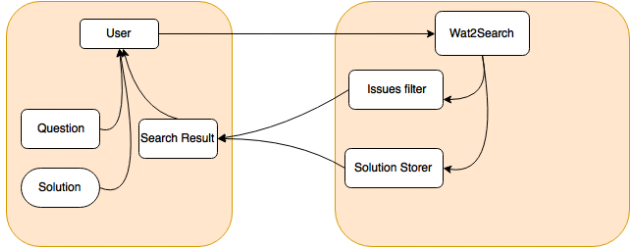
\includegraphics[scale=.75]{UML_oo.png}}

	\textbf{Packages:}
		\\\indent Our project is a web app designed to aid OSU users with solving technological issues. This web app may be its own web page or it may be an application that can be added like a widget to any web page. As our project is a web app, there are no OO entities to discuss. While javascript, the main functional language for websites, does support objects, it is not in the scope of our project to do so. For this section I will discuss how the app will be implemented, the “packages” so to speak, and coupling and cohesion of the parts of the app. It is important to note that using an object oriented language, or having an object oriented program was not a prerequisite for this project.
		
		The app will be programmed in javascript and designed using HTML and CSS. The app will have a homepage that will act as the starting point for the user. From their, the user will select which category they need help with. Animations will be programmed in javascript. These are not specifically coupled with anything. If anything, they are coupled with which buttons and categories we have. Coupling and cohesion refers to the functions within and between modules. As our application will not be programmed in such a way, it is not entirely useful. However, it will be discussed and related as closely as possible to our project. 
		
		After the user selects which path they will go on, they will be taken to a page for this path. This transition may be through traveling to a seperate HTML page or it may be through javascript. This has not been decided, but will be decided before implementation begins. In the case of using HTML pages, there would need to be many pages for each path a user may take. The links for these HTML pages would be coupled with the buttons that take the user to those locations. One path a user takes is independent of any other path. Because of this the pages are not related to each other, besides the links that may exist between the two.
		
		If our project is an independent website, our project will be hosted using a node.js runtime environment. This will be used to handle errors and serve the files to the users. There will be no database required for this web application as the different paths will be implemented manually and not pulled from a database. A database may speed up the process in a later version of this project. However, for the scope of this project, we will not use the database. This project will be the prototype for what the tool can be. Later, more information and paths the user can take will be added and updated frequently.
		

	\textbf{Design Patterns:}
	
\begin{enumerate}
	\item \textbf{Observer Pattern:}
	The observer pattern would be the most helpful because it can be applied to how the system reacts to the actions of the user.  For example, in response to a user selecting a category of issues the system will act accordingly by presenting new categories/questions to choose from.  When one object is changed, the other are update automatically. This allows for only relevant objects to be active as the user navigates the program. The system will display the new options in a visually comprehensive way, keeping with the chosen format for our user interface. The user’s actions will drive the program. So, the system will consistently listen for the user’s actions, reacting to the prompts provided, until they narrow down their concern/issue and receive instructions that will allow them to resolve their problem efficiently and precisely.  

	\item \textbf{Iterator Pattern:}
	Along with the observer pattern, this specific pattern could be useful in differentiating between the user’s direct interaction with the public interface and the underlying structure of the system and objects. For all intensive purposes, the program’s malleable technicalities will be under the hood as the user chooses the options on the surface level. The boolean variables used for the user choices will be signified visually as they interact with the program. While the program is recording their choices in an array of boolean variables, they build off of each other into a different array of bool vars based on the user choice. 
	
		\item \textbf{Proxy Pattern:}
	This pattern similarly will address the issue of reacting only the actions done by the user in which certain objects will be instantiated accordingly.  It doesn’t completely fit the description of our system, but it’s underlying idea can be applied and looked into for consideration in the designing and planning process.  Some of the actions the system will be looking for are the “clicking” upon an option that is displayed on the user interface or the option of going back to a previous category in the case they wrongly or accidently chose a category that doesn’t apply to their issue/problem.
	
		\item \textbf{Other Patterns:}
	Many of the other patterns are not applicable to our specific system because they involve a certain level of complexity we do not necessarily need to consider; as such with the builder pattern.  We will also not be working with a database and therefore do not need to take that into consideration. 
\end{enumerate}		
\textbf{Exceptions and Handling}
	\\Due to the nature of our application, the key exceptions that occur will be due to programming error or user error. If our application has an error in programming, such as a button to take a user from one page to the next is broken, then a correction needs to be done. As an exception cannot be thrown in a case like this, the complete functionality of our system will rely on users reporting issues and testing by us, the developers. Running through specific paths a user might take, such as with help resetting their ONID password, will allow us to confirm the functionality of our program. 
	The other type of exceptions that may occur is an error on the user’s side of the program. This type of error is based on the actions taken by the user. For example, again if the user wanted to reset their ONID password, they would select the Accounts category from the home page. However, let us say in this example that they select Networking. This is an error on their part and from their they cannot get to the information they are looking for. We will program buttons to handle such an error. On the bottom of the application, there are back and home buttons. The back button will take the user to the previous page, in this case the home page. The home button will take the user to the home page regardless of where they are within the application. Providing these two buttons will handle all user exceptions.
	
\textbf{Meeting Report:}
\\We once again met up at the Valley Library on campus at 1:00 p.m on Saturday to delineate who is assigned what task on this assignment. We also put some work into the assignment during our meeting, allowing us to agree upon the overall structure and cohesion of our work for this specific assignment. We voted earlier on a Doodle poll created by Evan that was useful in getting an idea of how everyone would be involved. But, wanted to elaborate further on what each task entailed. In the end, Donghao decided to do the UML Class Diagram. Lauren did the design patterns as well as looking over the meeting report. Robert decided to do the presentation slides since he had written the contents of the slides for the presentation in the beginning of the term. Luke covered the Packages portion of the assignment as well as the exceptions and handling portion. Evan decided to do the Meeting Report and the LaTex conversion once again while still providing supervision as a customer for the assignment. 
Throughout the week we communicated over Discord application. This mode of communication has been very useful in keeping up to date with each other. It is easily accessible for everyone and has provide to be very reliable and easy to navigate for those of us who haven’t used it before. To keep submissions consistent we used Robert’s GitHub for uploading all of our assignments. We also discussed uploading the second assignment again if we finished this one in time. In that discussion we talked about what may have been lacking in the initial submission.  Some issues we identified were missing requirements such as a bibliography file.  As a result, we were able to further determine what could be improved upon in the area of fleshing out our uses of the program. 
For next week, we want to get started on the technical side of actually putting the project together. During the meeting we also discussed further what workflow will be like when we’re actually programming the project. Luke and Donghao were eager to get started on this portion when we do begin that portion. Lauren displayed interest in the visual side of things. Robert and I will supervise and assist in every aspect where we can to make sure the project is how it was initially envisioned.

\end{document}
